\documentclass[a4paper, amsfonts, amssymb, amsmath, reprint, showkeys, showpacs, nofootinbib, twoside]{revtex4-2}
\usepackage[english]{babel}
\usepackage[utf8]{inputenc}
\usepackage[colorinlistoftodos, color=green!40, prependcaption]{todonotes}
\usepackage{bm}% bold math
\usepackage{amsthm}
\usepackage{mathtools}
\usepackage{physics}
\usepackage{xcolor}
\usepackage{graphicx}
\usepackage[left=23mm,right=13mm,top=35mm,columnsep=15pt]{geometry} 
\usepackage{adjustbox}
\usepackage{placeins}
\usepackage[T1]{fontenc}
\usepackage{lipsum}
\usepackage{csquotes}
\usepackage[pdftex, pdftitle={Article}, pdfauthor={Author}]{hyperref} % For hyperlinks in the PDF
%\setlength{\marginparwidth}{2.5cm}
\bibliographystyle{apsrev4-2}
\hypersetup{
    colorlinks=true,
    linkcolor=blue,
    citecolor=blue,
    urlcolor=blue
}

\begin{document}
\title{Collective Behavior, Chemotaxis and Chirality in Active Matter: A Review}

\author{Yichen Lu$^{1,2}$}
\author{Zhigang Zheng$^{1,3,}$}
\email{Corresponding author. zgzheng@hqu.edu.cn}

\affiliation{ 
$^1$Institute of Systems Science, Huaqiao University, Xiamen 361021, China\\
$^2$School of Mathematical Sciences, Huaqiao University, Quanzhou, 362021, China\\
$^3$College of Information Science and Technology, Huaqiao University, Xiamen 361021, China
}

\date{\today} % Leave empty to omit a date

\begin{abstract}
    Active matter systems, composed of self-propelled particles, chemotactic agents, and chiral particles exhibit a rich variety of collective behaviors driven by non-equilibrium dynamics. This review focuses on the modeling approaches in active matter, particularly emphasizing the roles of chemotaxis and chirality in shaping collective behaviors. We begin with particle-based models such as the Vicsek model and its variants, which capture the essential features of self-propelled particles and their interactions. We then explore chemotactic active particles and their interactions with chemical fields, highlighting the mechanisms of chemotaxis in shaping collective patterns. Hydrodynamic models provide a continuum description of active matter systems, revealing the emergent behaviors arising from microscopic interactions. Based on this, we analyze the stability of active matter systems, focusing on the role of chemotaxis and chirality in shaping collective behaviors. 
    Finally, we discuss the data-driven analysis of active matter systems, emphasizing the importance of machine learning techniques in understanding complex patterns and behaviors. The review aims to provide a comprehensive overview of the current state of research in active matter, focusing on the modeling approaches that have been developed to capture the essential features of self-propelled particles and their interactions.
\end{abstract}

\pacs{pacs}  % PACS, the Physics and Astronomy  % Classification Scheme.
\keywords{active matter, Vicsek model, chemotaxis, chirality, collective behavior}

\maketitle

\section{\label{sec:introduction}Introduction}

We live in a colorful world filled with systems composed of diverse individuals, spanning microscopic entities like bacteria \cite{Marchetti2015,PhysRevLett.104.178103} and colloidal Janus particles \cite{B718131K,doi:10.1021/cr300089t,Campbell2019,doi:10.1021/acs.accounts.8b00243} to macroscopic agents such as humans \cite{Majumdar_Pinsard_Nicolas_2020,PhysRevE.51.4282,Gu2025}, animals \cite{doi:10.1073/pnas.0711437105,Becker2015,doi:10.1073/pnas.1118633109,Qiu2015} and robots \cite{PhysRevLett.132.118301,PhysRevE.101.022603,Yangkai88703}. These systems exhibit a wide range of collective phenomena—from cell migration \cite{doi:10.1126/science.1209042,PhysRevLett.122.248102}, clustering \cite{PhysRevLett.110.238301,Ishimoto2018,C5SM01061F,Jinghan70501}, crystallization \cite{doi:10.1126/sciadv.aat7779,PhysRevE.97.052615}, lane formations \cite{PhysRevE.94.052603,Kogler_2015,C0SM01343A} to swirling formations \cite{PhysRevLett.100.058001,riedel2005self,PhysRevLett.93.098103,Daming60702}, low-Reynolds-number turbulence \cite{doi:10.1073/pnas.1710188114,PhysRevE.97.022613,PhysRevE.98.022603}, and even the emergence of negative viscosities \cite{annurev-fluid-010816-060049}. For instance, biological groups display behaviors like the swarming dynamics of bird flocks \cite{PhysRevLett.75.1226,doi:10.1073/pnas.1118633109,Qiu2015,PhysRevLett.119.058002} and the synchronized swimming of fish shoals \cite{doi:10.1073/pnas.0711437105,Becker2015}. Remarkably, such collective patterns extend beyond the scale of systems: superfluidity in bacterial teamwork \cite{Marchetti2015,PhysRevLett.104.178103} and collective oscillations in pedestrian crowds \cite{Majumdar_Pinsard_Nicolas_2020,PhysRevE.51.4282,Gu2025} reveal universal principles across scales. These behaviors not only inspire fascination but also hold profound implications for group survival and material science.

Active matter, a field that studies systems composed of self-propelled particles, has emerged as a powerful framework for understanding these collective behaviors. The term "active matter" refers to systems where individual components convert energy from their environment into motion, leading to non-equilibrium dynamics and emergent patterns. This review focuses on the modeling approaches in active matter, particularly emphasizing the roles of chemotaxis and chirality in shaping collective behaviors.
Active matter systems can be broadly categorized into two types: \textit{dry} active matter, where particles interact through short-range forces, and \textit{wet} active matter, where particles are immersed in a fluid medium. Dry active matter includes systems like self-propelled particles, flocking models, and granular materials, while wet active matter encompasses systems like swimming microorganisms, active colloids, and biofilms.
The study of active matter has gained significant attention in recent years, with a growing body of literature exploring various aspects of collective behavior, chemotaxis, and chirality. Theoretical models, numerical simulations, and experimental studies have all contributed to our understanding of these complex systems. This review aims to provide a comprehensive overview of the current state of research in active matter, focusing on the modeling approaches that have been developed to capture the essential features of self-propelled particles and their interactions.

The review is organized as follows. In Section~\ref{sec:models}, we discuss the modeling approaches in active matter, starting with particle-based models such as the Vicsek model and its variants. We then explore chemotactic active particles and their interactions with chemical fields. Section~\ref{sec:hydrodynamicModels} delves into hydrodynamic models of active matter, highlighting the continuum descriptions that emerge from microscopic interactions. In Section~\ref{sec:stabilityAnalysis}, we analyze the stability of active matter systems, focusing on the role of chemotaxis and chirality in shaping collective behaviors. We conclude with a summary of the key findings and future directions in active matter research. In Section~\ref{sec:DataDrivenAnalysis}, we discuss the data-driven analysis of active matter systems, emphasizing the importance of machine learning techniques in understanding complex patterns and behaviors. Finally, in Section~\ref{sec:Conclusion}, we summarize the key findings and highlight future directions for research in active matter.

\section{\label{sec:models}Modeling Approaches in Active Matter}

The theoretical foundation of active matter systems begins with particle-based models that capture the essential features of self-propelled particles and their interactions. Several paradigmatic models have emerged as standard frameworks for studying active matter phenomena. These models include the Vicsek model, which describes self-propelled particles with alignment interactions, and its variants that incorporate additional physical realism such as chemotaxis and chirality. In this section, we will discuss these models in detail, highlighting their key features and the insights they provide into collective behaviors.

\subsection{Vicsek Model and Its Variants}

The Vicsek model \cite{PhysRevLett.75.1226} represents one of the simplest yet most influential models for collective motion. It describes point particles moving at constant speed that align their directions of motion with neighbors within a fixed interaction radius. The model's dynamics are governed by:
\begin{subequations}
    \begin{align}
        \mathbf{x}_i\left( t+1 \right) &=\mathbf{x}_i\left( t \right) +\mathbf{v}_i\left( t \right) \Delta t\;,
        \\
        \theta_i \left( t+1 \right) &=\langle \theta \left( t \right) \rangle _r+\Delta \theta_i \;,
    \end{align}
\end{subequations}
where $\mathbf{x}_i$ is the position of particle $i$, $\mathbf{v}_i$ is its velocity, $\Delta t$ is the time step, $\theta_i$ is the orientation of particle $i$, $\langle \theta \left( t \right) \rangle _r$ is the average orientation of neighbors within a radius $r$, and $\Delta \theta_i$ is a random perturbation to account for noise. The Vicsek model has been extended to include various interactions, such as repulsion, attraction, and alignment, leading to rich phase diagrams and emergent behaviors, as illustrated in Fig.~\ref{fig:vicsekSnapshots}.

\begin{figure}
    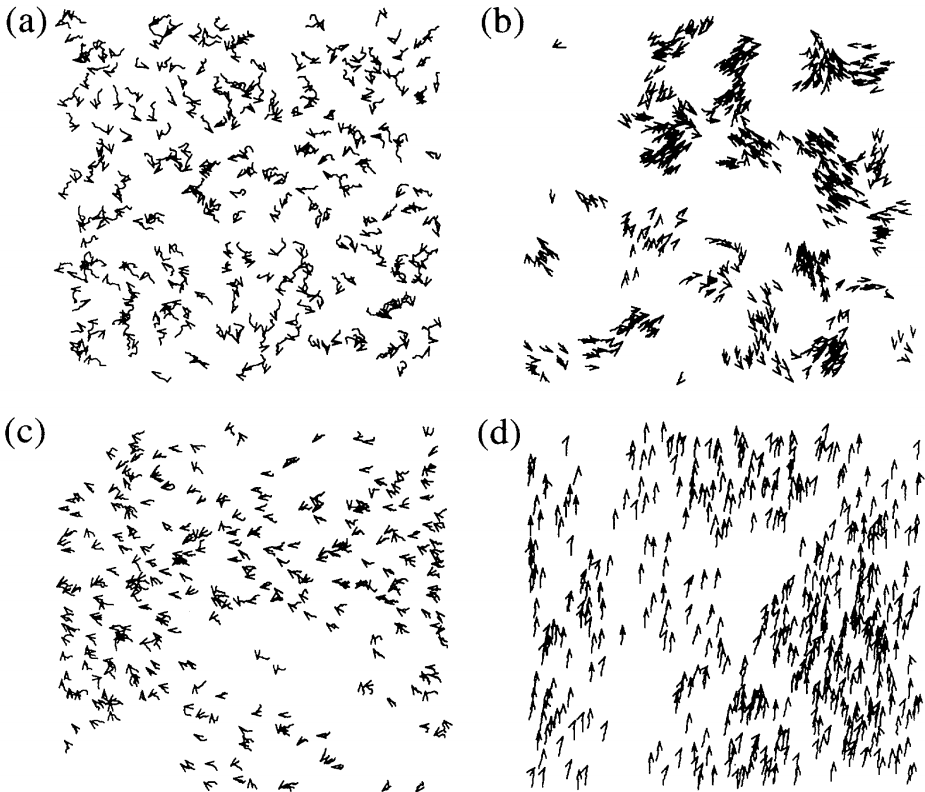
\includegraphics[width=0.49\textwidth]{./figs/vicsekSnapshots.png}
    \caption{
        \label{fig:vicsekSnapshots}
        In this figure the velocities of the particles are displayed for varying values of the density and the noise.
        The actual velocity of a particle is indicated by a small arrow, while their trajectory for the last 20 time steps is shown by a short continuous curve. he number of particles is $N = 300$ in each case. Copyright 2017 American Physical Society.
    }
\end{figure}

Recent extensions of the Vicsek model have incorporated additional physical realism:

\textbf{Self-propelled particles with Kuramoto-like alignment interaction:} Farrell et al. \cite{PhysRevLett.108.248101} introduced a self-propelled particle model with Kuramoto-like alignment interactions dependent on the particle density, where the dynamics are described by:
\begin{subequations}
    \begin{align}
        \dot{\mathbf{r}}_i&=v\mathbf{e}_{\theta _i}\;,
        \\
        \dot{\theta}_i&=\gamma \sum_{j=1}^N{F\left( \theta _j-\theta _i,\mathbf{r}_j-\mathbf{r}_i \right) +\sqrt{2\epsilon}\tilde{\eta}_i\left( t \right)}\;,
    \end{align}
\end{subequations}
where $\mathbf{r}_i$ is the position of particle $i$, $v$ is the self-propulsion speed, $\mathbf{e}_{\theta _i}$ is the unit vector in the direction of $\theta _i$, $\gamma$ is the alignment strength, $F$ is a function describing the interaction between particles, and $\tilde{\eta}_i\left( t \right)$ is a Gaussian white noise term. For simplicity, the authors choose $F\left( \theta ,\mathbf{r} \right) =\left( \pi R^2 \right) ^{-1}\sin \theta $ if $\left|\mathbf{r}\right|<R$ and 0 otherwise, where $R$ is the interaction radius. This model captures the essential features of collective motion while allowing for a tunable density-dependent alignment interaction. The phase diagram and the emergent patterns in this model exhibit rich behavior, including phase transitions between ordered and disordered states, as shown in Fig.~\ref{fig:ferrellSnapshots}.

\begin{figure}
    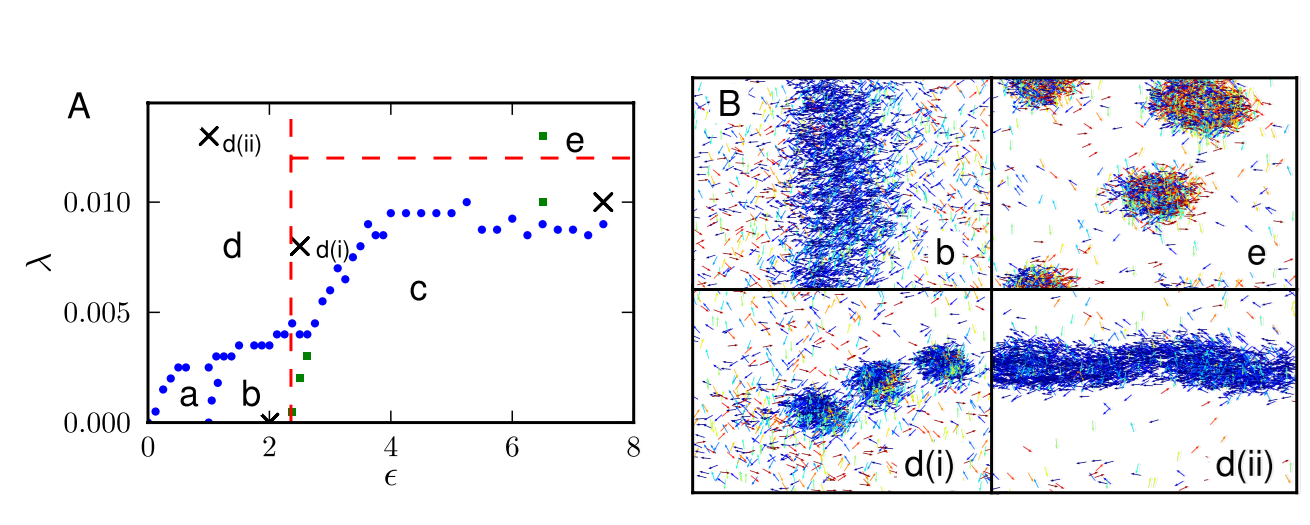
\includegraphics[width=0.49\textwidth]{./figs/Farrell.png}
    \caption{
        \label{fig:ferrellSnapshots}
        (A) Phase diagram in the $(\epsilon, \lambda)$ plane. Blue filled circles on the phase boundary correspond to peaks in the variance of the particle density, while green squares separate states with zero and nonzero mean orientation. Phases are labeled as per discussion in the text. Horizontal and vertical red lines indicate linear instabilities toward clustering and ordering, respectively.
        (B) Snapshots of the stripy (b), aster (e), moving clumps [d(i)], and lane [d(ii)] patterns. The crosses in A correspond to the snapshots in B. Particles are color coded by direction, with blue (darker gray) horizontal and red (lighter gray) vertical.
    }
\end{figure}

\textbf{Chiral active particles:} Liebchen and Levis \cite{PhysRevLett.119.058002} generalized the Vicsek model to include intrinsic rotations, described by:
\begin{subequations}
    \label{eq:chiralActiveParticles}
    \begin{align}
        \dot{\mathbf{r}}_i&=v\mathbf{p}_i \;,
        \\
        \dot{\theta}_i&=\omega +\frac{K}{\pi R_{\theta}^{2}}\sum_{j\in \partial _i}{\sin \left( \theta _j-\theta _i \right)}+\sqrt{2\epsilon}\tilde{\boldsymbol{\eta}}_i\left( t \right) \;,
    \end{align}
\end{subequations}
where $\omega$ is the natural rotation frequency, corresponding chirality of the particles, $K$ is the strength of the alignment interaction, $R_{\theta}$ is the interaction radius for orientation, and $\tilde{\boldsymbol{\eta}}_i\left( t \right)$ is a Gaussian white noise term. This model captures the essential features of chiral active particles, where the intrinsic rotation leads to a rich variety of collective behaviors, including phase separation and dynamic self-assembly. The phase diagram and the emergent patterns in this model exhibit rich behavior, including phase transitions between ordered and disordered states, as shown in Fig.~\ref{fig:2017Lieb}.
    
\begin{figure}
    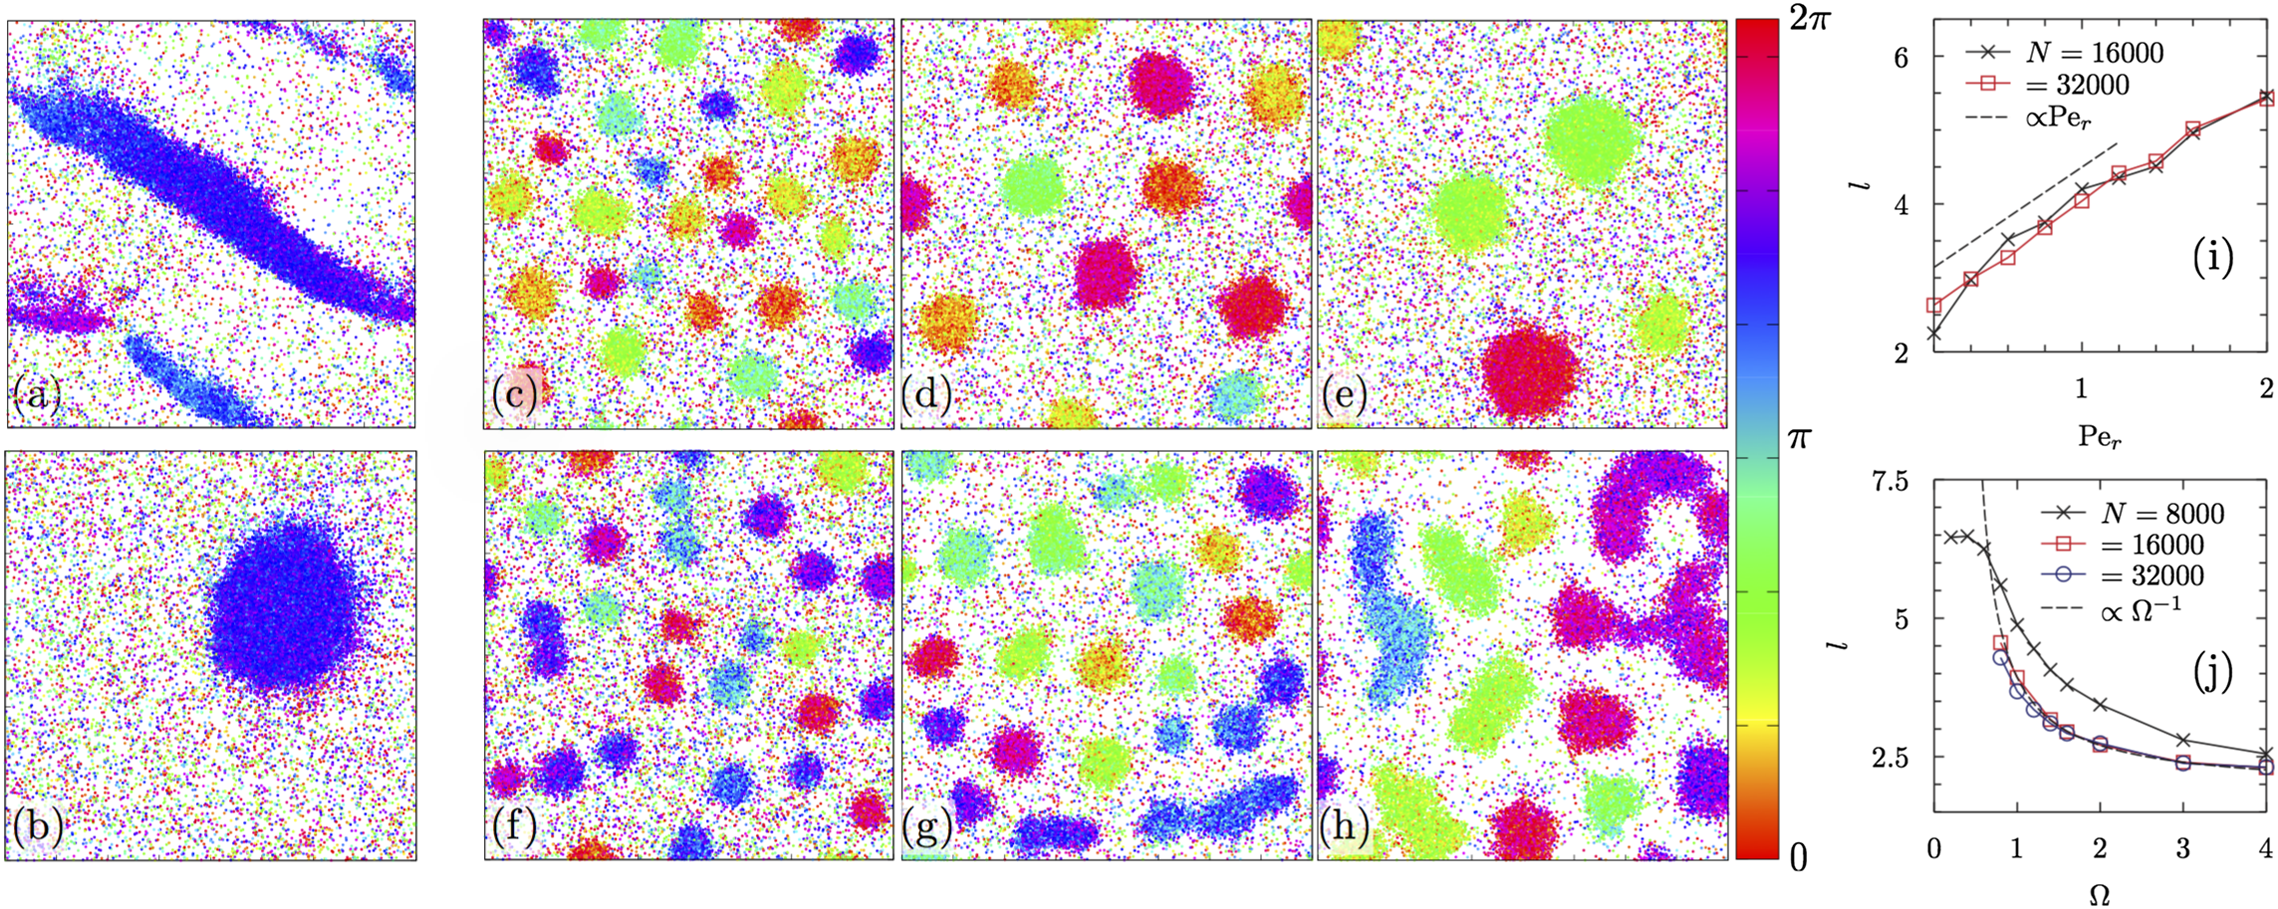
\includegraphics[width=0.49\textwidth]{./figs/2017Lieb.png}
    \caption{
        \label{fig:2017Lieb}
        Simulation snapshots for $N = 32000$ particles with colors encoding particle orientations. [(a), $\Omega = 0$]: Traveling bands;
        [(b), $\Omega = 0.2 < 1$]: rotating macrodroplet (phase separation) (c)–(h): Microflock pattern at $g\rho=2.8$, $\Omega=3$, and $\text{Pe}_r=0.2$ (c), $\text{Pe}_r=1$ (d), and $\text{Pe}_r=2$ (e), and at $\text{Pe}_r=0.2$, $\Omega=3$, and $g\rho=$ 2.4 (f), 3.6 (g), and 6 (h). (i), (j): Microflock length scale l for
        $g\rho=$ 2.8; for $\Omega=3$ as a function of Per (i), and for $\text{Pe}_r=0.2$ as a function of $\Omega$ (j) for the system sizes shown in the key.
    }
\end{figure}

\subsection{Chemotactic Active Particles}

Chemically interacting active particles exhibit rich pattern formation due to coupling between particle motion and chemical fields. The mechanism of chemotaxis is captured in the classical Keller--Segel model \cite{keller_initiation_1970,keller_model_1971}. The Langevin equation model of agent-based Keller--Segel model is defined as
\begin{subequations}
    \label{eq:agentsChemotaxis}
    \begin{align}
        &\dot{\mathbf{r}}_i(t)=\beta_D\nabla c(\mathbf{r}_1(t),t)+\sqrt{2D}\boldsymbol{\xi }(t)\;,\\
        &\dot{c}(\mathbf{r},t)=D_c\Delta c(\mathbf{r},t)+k_0\delta (\mathbf{r}-\mathbf{r}_i)-k_dc(\mathbf{r},t)\;,
    \end{align}
\end{subequations}
where $\mathbf{r}_i$ is the position of the $i$th particle, $c(\mathbf{r},t)$ is the concentration of the chemo-attractant, $\beta_D$ is the chemotactic sensitivity, which is a key parameter that determines the strength of the chemotactic response of the particles to the chemo-attractant.

\begin{figure}
    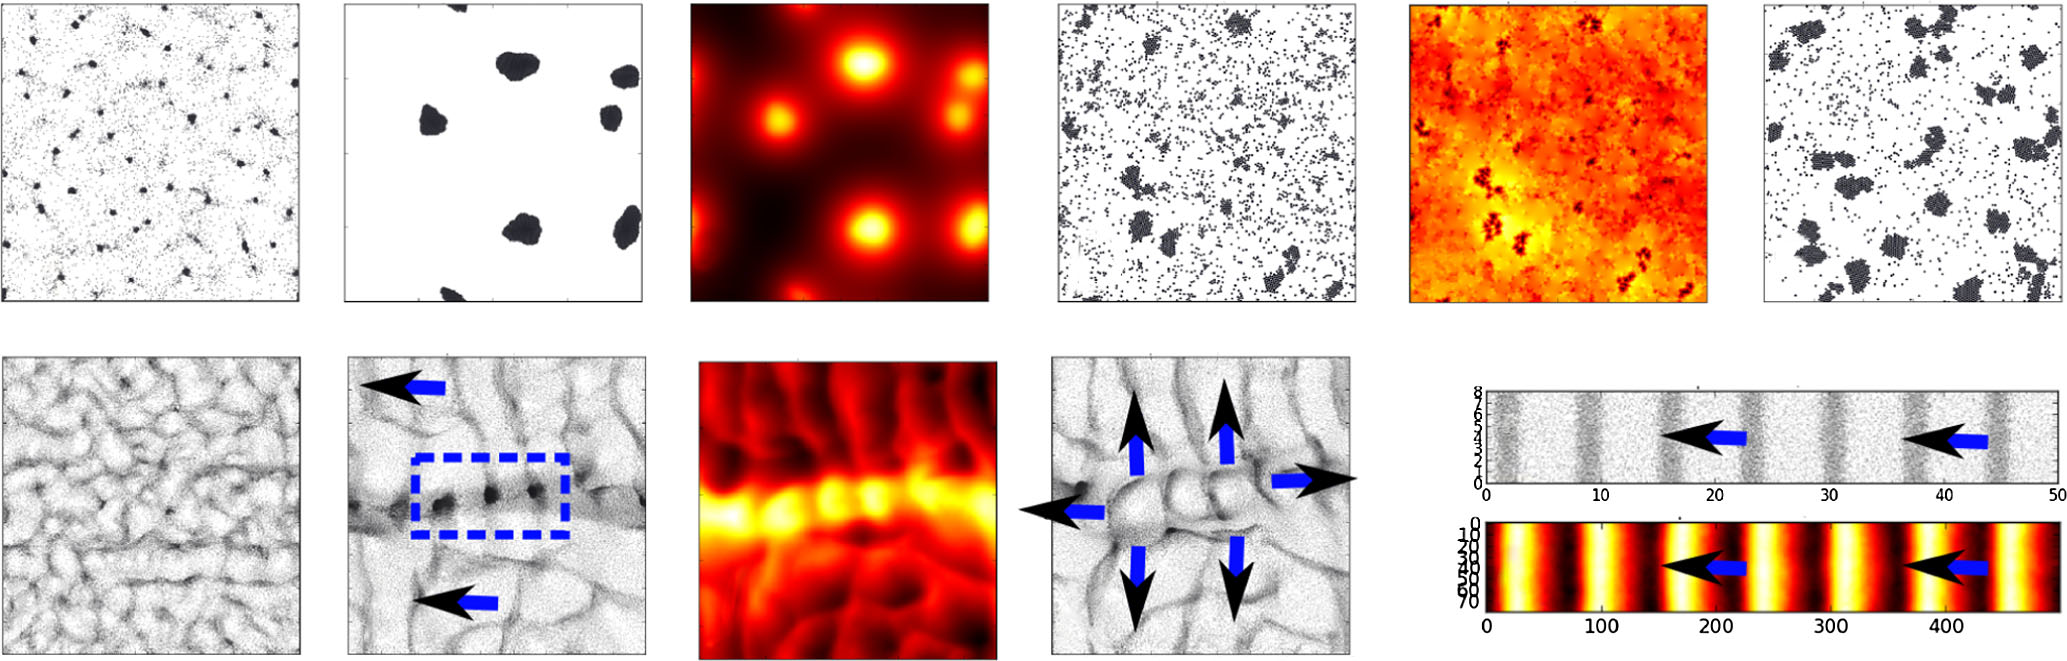
\includegraphics[width=0.49\textwidth]{./figs/chemoBehaviors1.png}
    \caption{
        \label{fig:chemoBehaviors1} Generic patterns in phoretic Janus colloids: snapshots from agent-based simulations.
        Reproduced with permission from ref.~\cite{PhysRevLett.118.268001}. Copyright 2017 American Physical Society.
    }
\end{figure}

When subjected to a chemical gradient, anisotropic particles—like self-propelled Janus colloids—can experience both displacement (a change in velocity) and alignment with or against the gradient (a change in self-propulsion direction). Essentially, this means they are influenced by both a force acting on their center of mass and a torque. The dynamics of such particles can be described by the motion of an overdamped chemotactic particle self-propelling with a velocity $v_0$ (independently of chemotaxis) in a direction $\mathbf{p}=\left(\cos\theta, \sin\theta\right)$ in two dimensions by the following evolution equations \cite{PhysRevLett.118.268001}
\begin{subequations}
    \label{eq:JanusChemotaxis}
    \begin{align}
        &\dot{\mathbf{r}}_i(t)=v_0\mathbf{p}_i\;,\\
        &\dot{\theta}_i(t)=\beta \mathbf{p}_i\times \nabla c(\mathbf{r}_i)+\sqrt{2D_{\mathbf{r}}}\xi _i(t)\;,\\
        &\dot{c}(\mathbf{r},t)=D_c\nabla ^2c(\mathbf{r},t)-k_dc(\mathbf{r},t)\notag\\
        &+\sum_{i=1}^N{\oint{\mathrm{d}\mathbf{x}_i\delta \left(\mathbf{r}-\mathbf{r}_i(t)-R_0\mathbf{x}_i\right)\sigma (\mathbf{x}_i)}}\;.
    \end{align}
\end{subequations}
The underlying physical mechanism is illustrated in Fig.~\ref{fig:chemoBehaviors1}. 

\section{\label{sec:hydrodynamicModels} Hydrodynamic Models of Active Matter}
At larger scales, continuum descriptions become essential for understanding active matter systems. Hydrodynamic theories provide powerful frameworks for analyzing the collective behaviors emerging from microscopic interactions. Here, we consider a general self-propelled particle system with short repulsive interactions and orientational alignment interactions, which is defined by the following equations:
\begin{subequations}
    \begin{align}
        &\dot{\mathbf{r}}_i\left( t \right) =v\mathbf{p}\left( \theta _i \right) +\sum_{j\ne i}{\mathbf{I}\left( \Delta \mathbf{r}_{ij} \right) }\;,\\
        &\dot{\theta}_i\left( t \right) =\omega _i +\sum_{j\ne i}{H\left( \Delta \theta _{ji},\Delta \mathbf{r}_{ij} \right)}\;,
    \end{align}
\end{subequations}
for $i=1,2,\cdots,N$. Here, $\mathbf{r}_i$ and $\theta _i$ is the position and orientation of the $i$-th particle, respectively,
$v$ is the self-propulsion velocity, $\mathbf{p}\left( \theta _i \right)=\left( \cos \theta _i,\sin \theta _i \right)$ is the instantaneous unit orientation, $\omega _i$ is the natural frequency, $H\left( \Delta \theta _{ij},\Delta \mathbf{r}_{ij} \right)$ is the coupling function between partials, $\Delta \mathbf{r}_{ij}=\mathbf{r}_i-\mathbf{r}_j$, $\Delta \theta _{ij}=\theta _i-\theta _j$.
\begin{eqnarray}
    &&\mathbf{I}\left( \Delta \mathbf{r} \right) =\frac{\Delta \mathbf{r}}{\left| \Delta \mathbf{r} \right|}k\left( R_r-\left| \Delta \mathbf{r} \right| \right) \Theta \left( R_r-\left| \Delta \mathbf{r} \right| \right) \\
    &&H\left( \Delta \theta ,\Delta \mathbf{r} \right) =K\sin \left( \Delta \theta \right) \Theta \left( R_{\theta}-\left| \Delta \mathbf{r} \right| \right) 
\end{eqnarray}

In the thermodynamic limit $N\rightarrow \infty$, the agent-based model gives rise to the following continuum form:
\begin{equation}
    \frac{\partial}{\partial t}f\left( \mathbf{r},\theta ,t \right) =-\frac{\partial}{\partial \theta}\left( fv_{\theta} \right) -\nabla \cdot \left( f\mathbf{v}_{\mathbf{r}} \right) \;, \label{eq:continuumModel}
\end{equation}
where $f\left( \mathbf{r},\theta ,t \right)$ is the probability density of particles at position $\mathbf{r}$ and orientation $\theta$ at time $t$, and $\mathbf{v}_{\mathbf{r}}$ and $v_{\theta}$ are the velocity fields in the position and orientation space, respectively. The velocity fields are given by
\begin{subequations}
    \small
    \begin{align}
        &v_{\theta}\left( \mathbf{r},\theta ,t \right) =\omega +K\int{\mathrm{d}\theta ^{\prime}f\left( \mathbf{r},\theta ^{\prime},t \right) \sin \left( \theta ^{\prime}-\theta \right)}\;,\\
        &\mathbf{v}_{\mathbf{r}}\left( \mathbf{r},\theta ,t \right) =v\mathbf{p}\left( \theta \right) +\int{\mathrm{d}\theta ^{\prime}\mathrm{d}\mathbf{r}^{\prime}f\left( \mathbf{r}^{\prime},\theta ^{\prime},t \right) \mathbf{I}\left( \mathbf{r}-\mathbf{r}^{\prime} \right) \;.}
    \end{align}
    \label{eq:velocityFields}
\end{subequations}
By substituting Eqs.~\eqref{eq:velocityFields} into Eq.~\eqref{eq:continuumModel}, we obtain
\begin{equation}
    \small
    \begin{aligned}
        \frac{\partial}{\partial t}f\left( \mathbf{r},\theta ,t \right) =&-v\mathbf{p}\left( \theta \right) \cdot \nabla f-\omega \partial _{\theta}f\\
        &-\nabla \cdot \left[ f\left( \mathbf{r},\theta ,t \right) \int{\mathrm{d}\theta ^{\prime}\mathrm{d}\mathbf{r}^{\prime}f\left( \mathbf{r}^{\prime},\theta ^{\prime},t \right) \mathbf{I}\left( \mathbf{r}-\mathbf{r}^{\prime} \right)} \right]\\
        &-K\partial _{\theta}\left[ f\left( \mathbf{r},\theta ,t \right) \int{\mathrm{d}\theta ^{\prime}f\left( \mathbf{r},\theta ^{\prime},t \right) \sin \left( \theta ^{\prime}-\theta \right)} \right] \;,\\
    \end{aligned}
\end{equation}
and we can rewrite it in a more compact form as
\begin{equation}
    \small
    \begin{aligned}
        \frac{\partial}{\partial t}f\left( \mathbf{r},\theta ,t \right) =&-v\mathbf{p}\left( \theta \right) \cdot \nabla f-\omega \partial _{\theta}f\\
        &-\nabla \cdot \left[ f\left( \mathbf{r},\theta ,t \right) \int{\mathrm{d}\theta ^{\prime}\mathrm{d}\mathbf{r}^{\prime}f\left( \mathbf{r}^{\prime},\theta ^{\prime},t \right) \mathbf{I}\left( \mathbf{r}-\mathbf{r}^{\prime} \right)} \right]\\
        &-K\partial _{\theta}\int{\mathrm{d}\theta ^{\prime}\mathrm{d}\mathbf{r}^{\prime}f\left( \mathbf{r},\theta ^{\prime},t \right) \sin \left( \theta ^{\prime}-\theta \right) \;,}\\
    \end{aligned}
\end{equation}
The equation accounts for self-propulsion, and short-range repulsion between particles, rotational diffusion and alignment interactions. 
From here, we expand $f\left( \mathbf{r},\theta ,t \right)$ in a Fourier series 
\begin{equation}
    f \left( \mathbf{r},\theta ,t \right) =\sum_{k=-\infty}^{\infty}{f _{k}\left( \mathbf{r},t \right) \mathrm{e}^{\mathrm{i}k\theta}}\;,
\end{equation} 
with the projection 
\begin{equation}
    \label{eq:fourierCoefficients}
    f _{k}\left( \mathbf{r},t \right) =\frac{1}{2\pi}\int{\mathrm{d}\theta f \left( \mathbf{r},\theta ,t \right) \mathrm{e}^{-\mathrm{i}k\theta}}\;,
\end{equation}

and define the coefficients  as the particle density $ \rho\left(\mathbf{r}, t\right)$ and the density-weighted polar order $\boldsymbol{p}\left(\mathbf{r}, t\right)$ by relating them to the harmonics via the Fourier expansion:
\begin{subequations}
    \small
    \begin{align}
        \rho \left( \mathbf{r},t \right) &\equiv \int_0^{2\pi}{\mathrm{d}\theta f\left( \mathbf{r},\theta ,t \right)}=2\pi f_{0}\left( \mathbf{r},t \right)
        \label{eq:particleDensity}
        \\
        \boldsymbol{p}\left( \mathbf{r},t \right) &\equiv \int_0^{2\pi}{\mathrm{d}\theta \mathbf{p}\left( \theta \right) f\left( \mathbf{r},\theta ,t \right)}\notag\\
        &=\int_0^{2\pi}{\mathrm{d}\theta \left[ \begin{array}{c}
        \cos \theta\\
        \sin \theta\\
    \end{array} \right] f\left( \mathbf{r},\theta ,t \right)}
    \notag \\
    &=\int_0^{2\pi}{\mathrm{d}\theta \frac{1}{2}\left[ \begin{array}{c}
        \mathrm{e}^{\mathrm{i}\theta}+\mathrm{e}^{-\mathrm{i}\theta}\\
        \mathrm{i}\left( \mathrm{e}^{-\mathrm{i}\theta}-\mathrm{e}^{\mathrm{i}\theta} \right)\\
    \end{array} \right] f\left( \mathbf{r},\theta ,t \right)}\notag\\
        &=\pi \left[ \begin{array}{c}
        f_{1}\left( \mathbf{r},t \right) +f_{-1}\left( \mathbf{r},t \right)\\
        \mathrm{i}\left( f_{1}\left( \mathbf{r},t \right) -f_{-1}\left( \mathbf{r},t \right) \right)\\
    \end{array} \right]
    \label{eq:polarOrder}
    \end{align}
\end{subequations}

In the following, the different contributions to the continuum model, are analyzed separately.

Firstly, in order to derive expressions for the self-propulsion, $-v\mathbf{p}\left( \theta \right) \cdot \nabla f$, we apply the projection operator, $f _{k}\left( \mathbf{r},t \right) =\frac{1}{2\pi}\int{\mathrm{d}\theta f \left( \mathbf{r},\theta ,t \right) \mathrm{e}^{-\mathrm{i}k\theta}}$, onto the corresponding term and obtain
\begin{equation}
    \tiny
    \begin{aligned}
        \frac{\partial}{\partial t}f_{k,\mathrm{prop}}=&\frac{1}{2\pi}\int_0^{2\pi}{\mathrm{d}\theta \mathrm{e}^{-\mathrm{i}k\theta}\left[ -v\mathbf{p}\left( \theta \right) \cdot \nabla f \right]}\\
        =&-\frac{v}{4\pi}\int_0^{2\pi}{\mathrm{d}\theta \left\{ \mathrm{e}^{-\mathrm{i}k\theta}\left[ \partial _x\sum_{m=-\infty}^{\infty}{f_m\left( \mathrm{e}^{\mathrm{i}\left( m+1 \right) \theta}+\mathrm{e}^{\mathrm{i}\left( m-1 \right) \theta} \right)} \right. \right.}\\
        &\left. \left. +\mathrm{i}\partial _y\sum_{k=-\infty}^{\infty}{f_m\left( \mathrm{e}^{\mathrm{i}\left( m-1 \right) \theta}-\mathrm{e}^{\mathrm{i}\left( m+1 \right) \theta} \right)} \right] \right\}\\
        =&-\frac{v}{2}\left\{ \partial _x\sum_{m=-\infty}^{\infty}{f_m\left[ \delta \left( m-k+1 \right) +\delta \left( m-k-1 \right) \right]} \right.\\
        &\left. +\mathrm{i}\partial _y\sum_{k=-\infty}^{\infty}{f_m\left[ \delta \left( m-k-1 \right) -\delta \left( m-k+1 \right) \right]} \right\} \;.\\
    \end{aligned}
\end{equation}

With the definitions of $\rho \left( \mathbf{r},t \right)$ and $\boldsymbol{p}\left( \mathbf{r},t \right)$, we obtain for the field variables
\begin{equation}
    \begin{aligned}
        \frac{\partial}{\partial t}\rho _{\mathrm{prop}}=&2\pi \frac{\partial}{\partial t}f_{0,\mathrm{prop}}\\
        =&-v\pi \left[ \partial _x\sum_{m=-\infty}^{\infty}{f_m\left( \delta _{m+1}+\delta _{m-1} \right)} \right.\\
        &\left. +\mathrm{i}\partial _y\sum_{k=-\infty}^{\infty}{f_m\left( \delta _{m-1}-\delta _{m+1} \right)} \right]\\
        =&-v\pi \left[ \partial _x\left( f_{-1}+f_1 \right) +\mathrm{i}\partial _y\left( f_1-f_{-1} \right) \right]\\
        =&-v\nabla \cdot \boldsymbol{p}_{\mathrm{prop}}\;,\\
    \end{aligned}
\end{equation}
and because of 
\begin{subequations}
    \begin{align}
        \partial _tf_{1}&=-\frac{v}{2}\left[ \partial _x\left( f_{0}+f_{2} \right) +\mathrm{i}\partial _y\left( f_{2}-f_{0} \right) \right] \;,\\
        \partial _tf_{-1}&=-\frac{v}{2}\left[ \partial _x\left( f_{0}+f_{2} \right) +\mathrm{i}\partial _y\left( f_{0}-f_{2} \right) \right] \;,
    \end{align}
\end{subequations}
we have
\begin{equation}
    \small
    \frac{\partial}{\partial t}\boldsymbol{p}_{\mathrm{prop}}=\pi \left[ \begin{array}{c}
        -v\partial _x\left( f_{0}+f_{2} \right)\\
        v\partial _y\left( f_{2}-f_{0} \right)\\
    \end{array} \right] \approx -\frac{v}{2}\left[ \begin{array}{c}
        \partial _xf_{0}\\
        \partial _yf_{0}\\
    \end{array} \right] =-\frac{v}{2}\nabla \rho _{\mathrm{prop}}
\end{equation}

Next, we turn to the rotational diffusion, $-\omega \partial _{\theta}f$. 
\begin{equation}
    \small
    \begin{aligned}
        \frac{\partial}{\partial t}f_{k,\mathrm{rota}}\left( \mathbf{r},t \right) &=-\frac{\omega}{2\pi}\int_0^{2\pi}{\mathrm{d}\theta \mathrm{e}^{-\mathrm{i}k\theta}\partial _{\theta}f\left( \mathbf{r},\theta ,t \right)}\\
        &=-\frac{\omega}{2\pi}\sum_{m=-\infty}^{\infty}{\mathrm{i}mf_{m,\mathrm{rota}}\left( \mathbf{r},t \right) \int_0^{2\pi}{\mathrm{d}\theta \mathrm{e}^{\mathrm{i}\left( m-k \right) \theta}}}\\
        &=-\omega \sum_{m=-\infty}^{\infty}{\mathrm{i}mf_{m,\mathrm{rota}}\left( \mathbf{r},t \right) \delta \left( m-k \right)}\\
        &=-\mathrm{i}k\omega f_{k,\mathrm{rota}}\left( \mathbf{r},t \right)\\
    \end{aligned}
\end{equation}
With the definitions of $\rho \left( \mathbf{r},t \right)$ and $\boldsymbol{p}\left( \mathbf{r},t \right)$, we obtain for the field variables
\begin{equation}
    \begin{aligned}
        \frac{\partial}{\partial t}\rho _{\mathrm{rota}}&=0\;,\\
        \frac{\partial}{\partial t}\boldsymbol{p}_{\mathrm{rota}}& =\omega \pi \left[ \begin{array}{c}
        \mathrm{i}\left( f_{-1,\mathrm{rota}}-f_{1,\mathrm{rota}} \right)\\
        f_{-1,\mathrm{rota}}+f_{1,\mathrm{rota}}\\
    \end{array} \right] =\omega \boldsymbol{p}_{\mathrm{rota},\bot}\;,\\
    \end{aligned}
\end{equation}
where $\boldsymbol{p}_{\mathrm{rota},\bot}=\left( -p_{\mathrm{rota},y},p_{\mathrm{rota},x} \right)$.

Next, we turn to the alignment interactions,
\begin{equation}
    \footnotesize
    \begin{aligned}
        \frac{\partial}{\partial t}f_{\mathrm{alig}}\left( \mathbf{r},\theta ,t \right) =&-K\partial _{\theta}\left[f\left( \mathbf{r},\theta ,t \right) \int{\mathrm{d}\theta ^{\prime}f\left( \mathbf{r},\theta ^{\prime},t \right) \sin \left( \theta ^{\prime}-\theta \right)}\right]\\
        =&K\mathrm{i}\pi \left( \mathrm{e}^{-\mathrm{i}\theta}f_{-1,\mathrm{alig}}-\mathrm{e}^{\mathrm{i}\theta}f_{1,\mathrm{alig}} \right) \sum_{-\infty}^{+\infty}{mf_{k,\mathrm{alig}}\mathrm{e}^{\mathrm{i}m\theta}}+\\
        &K\pi \left( \mathrm{e}^{-\mathrm{i}\theta}f_{-1,\mathrm{alig}}+\mathrm{e}^{\mathrm{i}\theta}f_{1,\mathrm{alig}} \right) f_{\mathrm{alig}}\\
    \end{aligned}
\end{equation}
and
\begin{widetext}
\begin{equation}
    \begin{aligned}
        \frac{\partial}{\partial t}f_{k,\mathrm{alig}}\left( \mathbf{r},t \right) =&\frac{1}{2\pi}\int{\mathrm{d}\theta f_{\mathrm{alig}}\left( \mathbf{r},\theta ,t \right) \mathrm{e}^{-\mathrm{i}k\theta}}\\
        =&-K\pi \left( f_{-1,\mathrm{alig}}\sum_{-\infty}^{+\infty}{mf_{k,\mathrm{alig}}\delta _{k-m+1}}-f_{1,\mathrm{alig}}\sum_{-\infty}^{+\infty}{mf_{k,\mathrm{alig}}\delta _{k-m-1}} \right)\\
        &+K\pi \left( f_{k+1,\mathrm{alig}}f_{-1,\mathrm{alig}}+f_{k-1,\mathrm{alig}}f_{1,\mathrm{alig}} \right)\\
        =&-K\pi \left[ \left( k+1 \right) f_{-1,\mathrm{alig}}f_{k,\mathrm{alig}}-\left( k-1 \right) f_{1,\mathrm{alig}}f_{k,\mathrm{alig}} \right]\\
        &+K\pi \left( f_{k+1,\mathrm{alig}}f_{-1,\mathrm{alig}}+f_{k-1,\mathrm{alig}}f_{1,\mathrm{alig}} \right)\\
    \end{aligned}
\end{equation}
\end{widetext}

With the definitions of $\rho \left( \mathbf{r},t \right)$ and $\boldsymbol{p}\left( \mathbf{r},t \right)$, we obtain for the field variables
\begin{equation}
    \begin{aligned}
        \frac{\partial}{\partial t}\rho _{\mathrm{alig}}&=0\;,\\
        \frac{\partial}{\partial t}\boldsymbol{p}_{\mathrm{alig}}&=\pi \left[ \begin{array}{c}
        \partial _t\left[ f_1\left( \mathbf{r},t \right) +f_{-1}\left( \mathbf{r},t \right) \right]\\
        \mathrm{i}\partial _t\left[ f_1\left( \mathbf{r},t \right) -f_{-1}\left( \mathbf{r},t \right) \right]\\
    \end{array} \right] =K\rho _{\mathrm{alig}}\boldsymbol{p}_{\mathrm{alig}}\\
    \end{aligned}
\end{equation}
because of
\begin{eqnarray}
    \begin{aligned}
        \frac{\partial}{\partial t}f_1&=K\pi \left( f_2f_{-1}+f_0f_1-2f_{-1}f_1 \right)\\
        &=K\pi f_1\left( f_0-2f_{-1} \right)\\
        \frac{\partial}{\partial t}f_{-1}&=K\pi \left( f_0f_{-1}+f_{-2}f_1-2f_{-1}f_1 \right)\\
        &=K\pi f_{-1}\left( f_0-2f_1 \right)\\
    \end{aligned}
\end{eqnarray}

Next, we turn to the short-range repulsion
\begin{widetext}
\begin{equation}
    \begin{aligned}
        \int{\boldsymbol{F}_{\mathrm{sr}}f\left( \mathbf{r}^{\prime},\theta ^{\prime},t \right) \mathrm{d}\mathbf{r}^{\prime}\mathrm{d}\theta ^{\prime}}&=2\pi \int{\frac{\mathbf{r}-\mathbf{r}^{\prime}}{\left| \mathbf{r}-\mathbf{r}^{\prime} \right|}k\left( R_r-\left| \mathbf{r}-\mathbf{r}^{\prime} \right| \right) \Theta \left( R_r-\left| \mathbf{r}-\mathbf{r}^{\prime} \right| \right) f\left( \mathbf{r}^{\prime},t \right) \mathrm{d}\mathbf{r}^{\prime}}\\
        &=2\pi \int_0^{R_r}{\int_0^{2\pi}{\mathbf{p}\left( \phi \right) k\left( R_r-d \right) \left[ f\left( 0,t \right) +d\nabla f\left( \mathbf{r}^{\prime},t \right) \right] \mathrm{d}d\mathrm{d}\phi}}\\
        &=\frac{4\pi ^2}{3}R_{r}^{4}\nabla f\left( \mathbf{r}^{\prime},t \right)\\
    \end{aligned}
\end{equation}
\end{widetext}
where $\boldsymbol{F}_{\mathrm{sr}}$ is the short-range repulsion force, $R_r$ is the interaction radius, and $k\left( R_r-\left| \mathbf{r}-\mathbf{r}^{\prime} \right| \right)$ is the strength of the short-range repulsion. The interaction radius $R_r$ is a key parameter that determines the strength of the short-range repulsion. The short-range repulsion can be positive or negative, depending on the nature of the interaction. If the interaction is attractive, the short-range repulsion is negative, and the particles move toward each other. If the interaction is repulsive, the short-range repulsion is positive, and the particles move away from each other.

To summarize, the continuum model can be written as
\begin{subequations}
    \begin{align}
        &\dot{\rho}^{1,2}\left( \mathbf{r},t \right) =-v\nabla \cdot \boldsymbol{p}^{1,2}+D\nabla ^2\rho ^{1,2}\;,\\
        &\dot{\boldsymbol{p}}^{1,2}\left( \mathbf{r},t \right) =-\frac{v}{2}\nabla \rho ^{1,2}+D\nabla ^2\boldsymbol{p}^{1,2}+\omega \boldsymbol{p}_{\bot}^{1,2}-K\rho\boldsymbol{p}\;,
    \end{align}
\end{subequations}

\section{\label{sec:stabilityAnalysis} Stability Analysis of Hydrodynamic Models}
Here, we analyse the stability of the hydrodynamic model of active matter with a simple example of Keller--Segel type chemotaxis in Eq.~\eqref{eq:agentsChemotaxis}. 
Based on the hydrodynamic theory, the macroscopic equations for the system in Eqs.~\eqref{eq:agentsChemotaxis} with the density $\rho (\mathbf{r},t)$ and the concentration $c(\mathbf{r},t)$ of the chemo-attractant are given by
\begin{subequations}
    \label{eq:hydroChemotaxis}
    \begin{align}
        &\dot{\rho}\left( \mathbf{r},t \right) =-\nabla \cdot \left( \beta _D\rho \left( \mathbf{r},t \right) \nabla c\left( \mathbf{r},t \right) \right) +D\nabla ^2\rho \left( \mathbf{r},t \right)\\
        &\dot{c}\left( \mathbf{r},t \right) =D_c\nabla ^2c\left( \mathbf{r},t \right) +k_0\rho \left( \mathbf{r},t \right) -k_dc\left( \mathbf{r},t \right)\;.
    \end{align}
\end{subequations}
These equations represent the classical Keller--Segel model. The chemotactic sensitivity $\beta _D$ is a key parameter that determines the strength of the chemotactic response of the particles to the chemo-attractant. The chemotactic sensitivity can be positive or negative, depending on the nature of the chemo-attractant. If the chemo-attractant is attractive, the chemotactic sensitivity is positive, and the particles move toward regions of higher chemo-attractant concentration. If the chemo-attractant is repulsive, the chemotactic sensitivity is negative, and the particles move away from regions of higher chemo-attractant concentration.

One obvious solution of Eqs.~\eqref{eq:hydroChemotaxis} is $(\rho, c)=(\rho_0, k_0\rho_0/k)$ representing a uniform disordered phase. Performing a linear stability analysis of this phase, we introduce small perturbations $\delta \rho$ and $\delta c$ around the uniform solution:
\begin{equation}
    \rho =\rho _0+\delta \rho , c=c_0+\delta c\,\,\left( \left| \delta \rho \right|\ll \rho _0, \left| \delta c \right|\ll c_0 \right) \;,
\end{equation}
and linearize Eqs.~\eqref{eq:hydroChemotaxis} to obtain
\begin{subequations}
    \begin{align}
        \dot{\delta}\rho &=-\beta _D\nabla \cdot \left( \rho \nabla \delta c \right) +D\nabla ^2\delta \rho\notag \\
        &=-\beta _D\nabla \cdot \left[ \left( \rho _0+\delta \rho \right) \nabla \left( c_0+\delta c \right) \right] +D\nabla ^2\left( \rho _0+\delta \rho \right)\notag \\
        &=D\nabla ^2\delta \rho -\beta _D\rho _0\nabla ^2\delta c-\beta _D\nabla \cdot \underset{\approx 0}{\underbrace{\left( \delta \rho \nabla \delta c \right) }}\notag \\
        &=D\nabla ^2\delta \rho -\beta _D\rho _0\nabla ^2\delta c \;,\\
        \dot{\delta}c&=D_c\nabla ^2\delta c+k_0\delta \rho -k_d\delta c+\underset{=0}{\underbrace{k_0\delta _0-k_dc_0}}\notag \\
        &=D_c\nabla ^2\delta c+k_0\delta \rho -k_d\delta c \;.
    \end{align}
\end{subequations}
Then we take the form of a plane wave:
\begin{subequations}
    \begin{align}
        \delta \rho =\delta \rho _0\mathrm{e}^{\sigma t+\mathrm{i}\mathbf{k}\cdot \mathbf{r}}, 
        \\
        \delta c=\delta c_0\mathrm{e}^{\sigma t+\mathrm{i}\mathbf{k}\cdot \mathbf{r}}\;,
    \end{align}
\end{subequations}
where $\sigma$ is the growth rate of the perturbation, $\mathbf{k}$ is the wave vector, and $\delta \rho _0$ and $\delta c_0$ are the amplitudes of the perturbations. Substituting these expressions into the linearized equations, we obtain
\begin{subequations}
    \begin{align}
        \sigma \delta \rho _0&=-Dk^2\delta \rho _0+\beta _D\rho _0k^2\delta c_0\;,\\
        \sigma \delta c_0&=-D_ck^2\delta c_0+k_0\delta \rho _0-k_d\delta c_0\;,
    \end{align}
    \label{eq:linearStability}
\end{subequations}
which can be written in matrix form as
\begin{equation}
    \left( \begin{array}{cc}
        \sigma +Dk^2 & -\beta _D\rho _0k^2\\
        -k_0 & \sigma +D_ck^2+k_d\\
    \end{array} \right) \left( \begin{array}{c}
        \delta \rho _0\\
        \delta c_0\\
    \end{array} \right) =0\;.
\end{equation}
In order for this system to have non-trivial solutions, the determinant of the matrix must be zero:
\begin{equation}
    \det \left( \begin{matrix}
        \sigma +Dk^2&		-\beta _D\rho _0k^2\\
        -k_0&		\sigma +D_ck^2+k_d\\
    \end{matrix} \right) =0
\end{equation}
This is a quadratic equation in $\sigma$, to let $\sigma < 0, \forall k=\left|\bf{k}\right|$ , we need to have
\begin{equation}
    \forall k, \begin{cases}
        \left( D+D_c \right) k^2+k_d>0\\
        DD_ck^4+\left( Dk_d-\beta _D\rho _0k_0 \right) k^2>0\\
    \end{cases} \;,
\end{equation}
which is satisfied for all $k$ if
\begin{equation}
    Dk_d>\beta _D\rho _0k_0\;.
\end{equation}
This is the Keller--Segel instability, which occurs for chemoattraction ($\beta_D>0$) and a sufficiently high chemoattractant production rate $k_0$. The instability leads to the formation of spatial structures in the density field $\rho(\mathbf{r},t)$ and the chemo-attractant concentration field $c(\mathbf{r},t)$, as shown in Fig.~\ref{fig:schematicPlot1}. Key metrics for characterizing collective states include:

\begin{figure}
    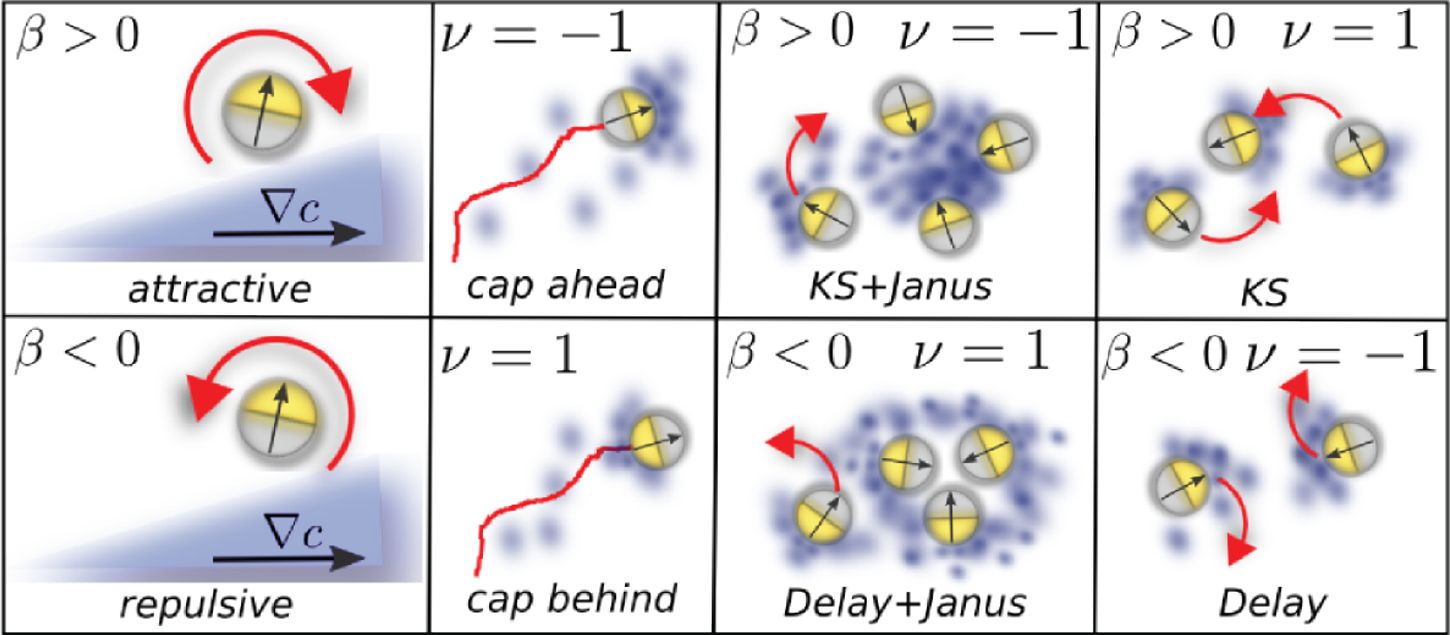
\includegraphics[width=0.49\textwidth]{./figs/schematicPlot1.png}
    \caption{
        \label{fig:schematicPlot1} Schematic plot of the chemotactic response of active particles to a chemo-attractant. Here, KS represents the Keller--Segel instability, and Janus and Delay stand for the Janus instability and the delay induced instability discussed in the text. Reproduced with permission from ref.~\cite{PhysRevLett.118.268001}. Copyright 2017 American Physical Society.
    }
\end{figure}

\section{\label{sec:DataDrivenAnalysis} Data-Driven Analysis of Collective Behaviors}

Advances in imaging and tracking technologies have enabled quantitative characterization of natural and synthetic active systems, facilitating data-driven approaches to understanding collective dynamics.

\begin{figure}
    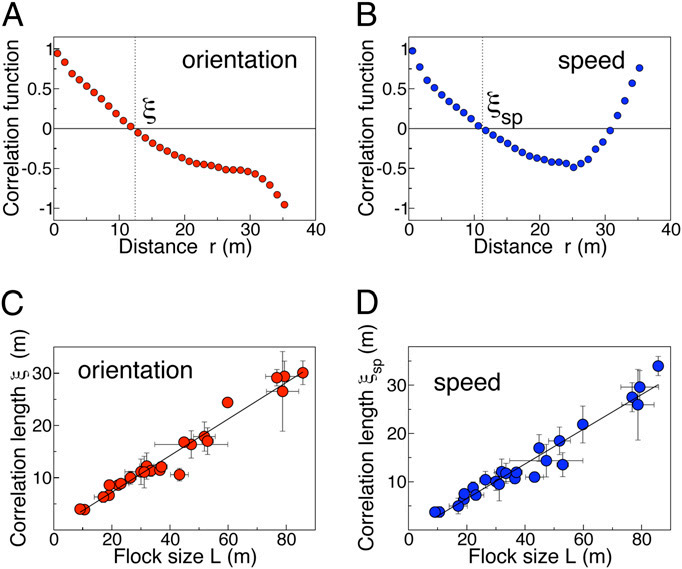
\includegraphics[width=0.49\textwidth]{./figs/VelocityCorr.png}
    \caption{
        \scriptsize
        \label{fig:velocityCorr}
        (A) The correlation function $C(r)$ is the average inner product of the velocity fluctuations of pairs of birds at mutual distance $r$. This correlation function therefore measures to what extent the orientations of the velocity fluctuations are correlated. The function changes sign at $r = \xi$, which gives a good estimate of the average size of the correlated domains (flock 28-10).
        (B) The correlation function $C_{sp}(r)$, on the other hand, measures the correlations of the fluctuations of the modulus of the velocity, i.e., the speed. This correlation function measures to what extent the variations with respect to the mean of the birds' speed are correlated to each other. The speed correlation function changes sign at a point $r = \xi_{sp}$, which gives the size of the speed-correlated domains (flock 28-10). Both correlation functions in (A) and (B) are normalized to give $C(r=0)=1$.
        (C) The orientation correlation length $\xi$ is plotted as a function of the linear size $L$ of the flocks. Each point corresponds to a specific flocking event, and it is an average over several instants of time in that event. Error bars are SDs. The correlation length grows linearly with the size of the flock, $\xi=aL$, with $a=0.35$ (Pearson's correlation test: $n=24$, $r=0.98$, $P<10^{-16}$), signaling the presence of scale-free correlations.
        (D) Also in the case of the correlation function of the speed, the correlation length $\xi_{sp}$ grows linearly with the size of the flock, $\xi_{sp}=aL$, with $a=0.36$ (Pearson's correlation test: $n=24$, $r=0.97$, $P<10^{-15}$). Error bars are SDs.
    }
\end{figure}

\begin{figure}
    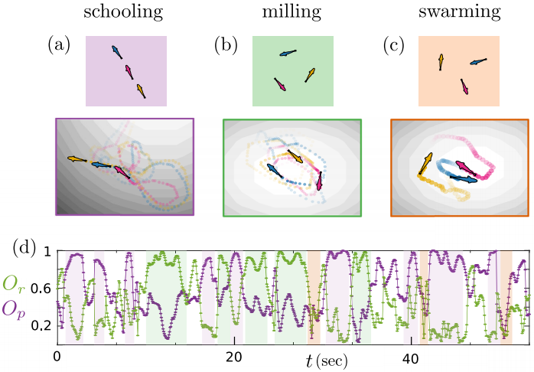
\includegraphics[width=0.49\textwidth]{./figs/rotationalOrderParameter.png}
    \caption{
        \label{fig:rotationalOrderParameter}
        Three fish exhibit schooling, milling and swarming states. Sketched and example experimental trajectories of the different dynamical states of three fish (a)
        schooling, (b) milling and (c) swarming. d Time evolution of the rotational and polarization order parameters $O_r$ and $O_p$ respectively.
    }
\end{figure}

\begin{figure}
    \centering
    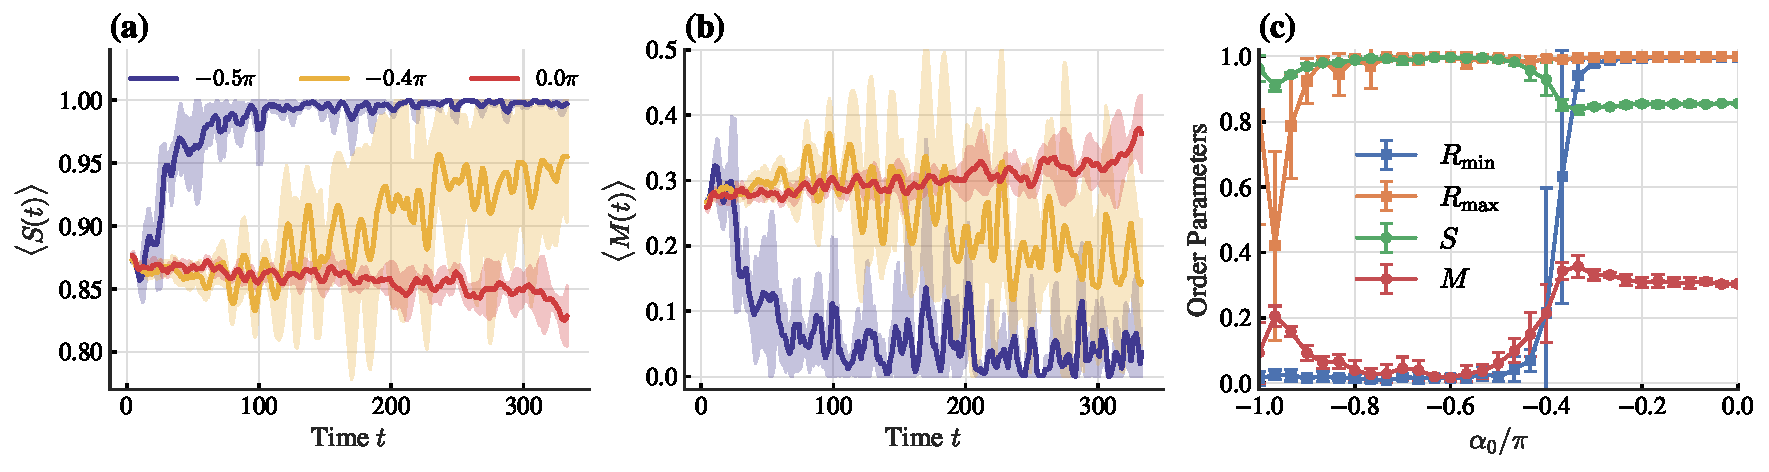
\includegraphics[width=0.49\textwidth]{./figs/orderParameters.pdf}
    \caption{
        \label{fig:orderParameters} 
        The time evolution of order parameters and their dependence on phase frustration $\alpha_0$.
        \textbf{(a--b)}, time evolution of the order parameters $S$ and $M$ for different phase frustration $\alpha_0$, where \enquote{$\langle\cdot\rangle$} denotes the average taken over the minimal frequency $\omega_{\min}\in\left[10^{-3}, 0.5\right]$.
        \textbf{(c)}, order parameters $S$, $M$, $R_{\max}$ and $R_{\min}$ versus $\alpha_0$ averaged over different initial conditions for $\omega_{\min}=10^{-3}$.
        (translucent bond and error-bars representing the standard deviation of values with different minimal frequencies and initial conditions, respectively).
    }
\end{figure}

\textbf{Velocity correlation function:}
Cavagna et al. introduced the velocity correlation function to quantify collective motion in flocks of birds~\cite{doi:10.1073/pnas.1005766107}. It is defined as
\begin{equation}
    C\left( r \right) =\frac{1}{c_0}\frac{\sum\nolimits_{ij}^{}{\vec{u}_i\cdot \vec{u}_j\delta \left( r-r_{ij} \right)}}{\sum\nolimits_{ij}^{}{\delta \left( r-r_{ij} \right)}}\;,
\end{equation}
where $\vec{u}_i=\vec{v}_i-N^{-1}\sum\nolimits_{k=1}^N{\vec{v}_k}$, $\vec{v}_i$ is the velocity of particle $i$, $r_{ij}=\left| \vec{r}_i-\vec{r}_j \right|$ is the distance between particles $i$ and $j$, and $c_0$ is a normalization constant. The velocity correlation function captures the spatial structure of collective motion, with positive values indicating alignment and negative values indicating anti-alignment, as illustrated in Fig.~\ref{fig:velocityCorr}(A). The correlation length $\xi$ is defined as the distance at which $C(r)$ changes sign, indicating the scale of correlated motion.

\textbf{Ploar and Rotational order parameter:} Zampetaki et al. \cite{Zampetaki2024} introduced the polar order parameter $O_p$ and the rotational order parameter $O_r$ to quantify the degree of alignment in collective motion. The polar order parameter is defined as
\begin{equation}
    O_p=\frac{1}{N}\left| \sum_{i=1}^N{\frac{\mathbf{v}_i}{\left| \mathbf{v}_i \right|}} \right|\;,
\end{equation}
where $\mathbf{v}_i$ is the velocity of particle $i$. The polar order parameter captures the degree of alignment of the particles' velocities, with $O_p=1$ indicating perfect alignment and $O_p=0$ indicating complete disorder.
The rotational order parameter is defined as
\begin{equation}
    O_r=\frac{1}{N}\left| \sum_{i=1}^N{\frac{\mathbf{v}_i}{\left| \mathbf{v}_i \right|}}\times \left( \frac{\mathbf{r}_i-\mathbf{r}_{\mathrm{cm}}}{\left| \mathbf{r}_i-\mathbf{r}_{\mathrm{cm}} \right|} \right) \right|\;,
\end{equation}
where $\mathbf{r}_{\mathrm{cm}}$ is the center of mass of the system. The rotational order parameter captures the degree of rotation in the collective motion, with $O_r=1$ indicating perfect rotation and $O_r=0$ indicating no rotation. These order parameters are illustrated in Fig.~\ref{fig:rotationalOrderParameter}(d).

\textbf{Order parameters of phase separation:} Firstly, an order parameter to measure the chiral demixing among particles can be defined as:
\begin{equation}
    S\left( t \right) =\frac{1}{N}\sum_{i=1}^N{\frac{\sum_{j\in A_i}{H\left( \omega _i\omega _j \right)}}{\left| A_i\left( t \right) \right|}}\;,
\end{equation}
where $H\left( x \right) =\left( x>0 \right)$ is the Heaviside step function. $S\left( t \right)$ is the fraction of the pairs of neighboring particles with the same chirality. When $S\left( t \right)=1$, all neighboring pairs share chirality, and the system is in a completely phase-separated state. When $S\left( t \right)< 1$, the system is in a mixed state.
Except for measuring the demixing degree, an order parameter to measure the degree of the complete demixing can be defined as:
\begin{equation}
    M\left( t \right) =\frac{1}{N}\sum_{i=1}^N{H\left[ \sum\nolimits_{j\in A_i}^{}{H\left( -\omega _i\omega _j \right)} \right]}\;.
\end{equation}
$M\left( t \right)$ is the fraction of particles that have neighbors with different chirality. When $M\left( t \right)=0$, the system is completely phase-separated. When $M\left( t \right)> 0$, the system is in a mixed state. Obviously, $M$ describes the qualitative nature of the complete demixing of the system, while $S$ describes the partial demixing, which is a more loose measure.
The above order parameters measure the chiral demixing from the perspective of the spatial distribution. 
The coordination of the internal phases can also be quantified to describe the demixing of the system. Firstly, a usual order parameter to measure the phase synchronization of the system can be defined as: 
\begin{equation}
    Z\left( t \right) =R\left( t \right) \mathrm{e}^{\mathrm{i}\psi \left( t \right)}=\frac{1}{N}\sum_{j=1}^N{\mathrm{e}^{\mathrm{i}\theta _j\left( t \right)}}\;,
\end{equation}
where $\textrm{i}=\sqrt{-1}$. The degree modulus $R(t)=\left|Z(t)\right|$ is the absolute value of the mean of the complex numbers $e^{\textrm{i}\theta _i}$, which can be interpreted as the absolute value of the mean normalized velocity of all particles. When $R\approx 1$, particles are fully phase synchronized, and when $R\approx0$, particles are phase incoherent.
In a mixed state, the partials are phase locked with each other, and the order parameter $R$ remains constant in the long run, while for the phase-separated state, the particles of different chiralities are uncoupled, then $R$ will fluctuate over time. These behaviors can be quantified by the maximum and minimum values of $R$ in a certain time window:
\begin{subequations}
    \begin{align}
        R_{\max}&=\max_{t\in W} \left\{ R\left( t \right) \right\} 
        \\
        R_{\min}&=\min_{t\in W} \left\{ R\left( t \right) \right\} 
    \end{align}
\end{subequations}
where $W=\left[ T-h,T+h \right]$ is a time window that is long enough to cover the transient and steady states of the system. When $R_{\max}=R_{\min}\approx1$, the system is in a mixed state, and when $R_{\max}\neq R_{\min}$, the system is phase-separated. As shown in Fig.~\ref{fig:orderParameters}, the order parameters $S$, $M$, $R_{\max}$ and $R_{\min}$ can be used to characterize the phase separation of the system. The order parameters $S$ and $M$ are sensitive to the degree of demixing, while $R_{\max}$ and $R_{\min}$ are sensitive to the coordination of the internal phases.

\section{\label{sec:Conclusion} Conclusion and Outlook}

The study of active matter has profoundly expanded our understanding of nonequilibrium statistical physics while providing frameworks for designing bio-inspired materials and robotic systems. From fundamental particle models to continuum theories and data-driven analyses, researchers have developed a rich toolkit for investigating and controlling collective behaviors in active systems.

The interplay between activity, interactions, and external fields continues to reveal new phenomena, such as phase separation, flocking, and pattern formation. Future research will likely focus on integrating machine learning techniques to analyse complex data sets, exploring the role of noise and disorder in active matter, and developing novel materials with tunable collective properties.

Future progress will likely come from combining theoretical insights with data-driven approaches and experimental advances, promising to unveil new principles of emergent organization in nonequilibrium systems. The interdisciplinary nature of active matter research positions it to make transformative contributions across physics, biology, and engineering in the coming years. 

\begin{acknowledgments}
This work is partially supported by The Nonlinear Dynamics Research Group led by Professor Zheng and Institute of Systems Science, Huaqiao University, Xiamen.
\end{acknowledgments}

\bibliography{ref}

\end{document}
